\documentclass[12pt]{article}
\usepackage{amsmath, amssymb}
\usepackage{bbold}
\usepackage{graphicx}
\graphicspath{{images/}}
\usepackage[top = 2.5cm, bottom = 2.5cm, left = 2.5cm, right = 2.5cm]{geometry}
\usepackage{natbib} % To cite
\usepackage[ruled,vlined]{algorithm2e}
\title{Coalescence manuscript}

\begin{document}
	\maketitle
	\section{Model}
	Consider the model presented in \cite{Marsland2019}, and let me make the following assumptions: (1) all resources contain the same amount of energy (taken to be 1 for simplicity), (2) a type I functional response, (3) a binary matrix of consumer preferences, and (4) externally supplied resources\\
	This assumptions correspond to the following model
	\begin{equation}\label{hybrid}
		\begin{aligned}
		\frac{dn_i}{dt} &= g_in_i\left(\sum_j(1-l_j)c_{ij}R_j - m_i\right)\\
		\frac{dR_{j}}{dt} &= \kappa_j - \tau^{-1}_jR_j - \sum_in_ic_{ij}R_j + \sum_{ik}n_iD_{kj}l_kc_{ik}R_k
		\end{aligned}
	\end{equation}
	where $ n_i $ is the population of species $ i $ and $ g_i $ is a proportionality constant relating energy to abundance of strain $ i $. The growth of species $ i $ is determined by the resources it harvests, which in turn depends on the resource concentration $ R_j $, and whether or not the species $ i $ consumes resournce $ j $ ($ c_{ij} = 1 \text{ or } c_{ij} = 0 $ respectively). However, not all the harvested resources contribute to growth. A fraction of them, $  l_j $, leak back to the environment as metabolic by-products. Additionally, species $ i $ invests some of the harvest in its living maintenance cost $ m_i $. The remaining resources after subtracting secretions and maintenance are transformed into biomass. \par 
	$ R_j $ is the concentration of resource $ j $. $ \kappa_j $ and $ \tau_j^{-1} $ encode the external dynamics of the resources; they are the supply and dilution rate of resource  $ j $, respectively. $ l_k $ is the leakage fraction ($ 0 < l_k < 1 $), and $ D_{jk} $ represents the metabolic matrix, ie, the fraction of resource $ j $ that is transformed into resource $ k $. Note that the rows of $ D $ sum to 1.  \par
	This model can be conveniently expressed in matrix form  as follows
	\begin{equation}
		\begin{aligned}
		\frac{d\boldsymbol{n}}{dt} &= \boldsymbol{g}\circ \boldsymbol{n}\left(D(\boldsymbol{R})C(\boldsymbol{1}-\boldsymbol{l}) - \boldsymbol{m}\right)\\
		\frac{d\boldsymbol{R}}{dt} &= \kappa - D(\boldsymbol{R})\boldsymbol{\tau}^{\circ -1}- D(\boldsymbol{R})C^T\boldsymbol{n} + D^TD(\boldsymbol{l}\circ \boldsymbol{R})C^T\boldsymbol{n}
		\end{aligned}
	\end{equation}
	where bold symbols are vectors and $ \circ $ denotes element-wise  operation\par
	If I further assume (5) that the dilution all resources is slow, that is, $ \tau_j^{-1} << 1$ then the resource dynamics can be assumed to be at steady state, and a time scale separation between resource and population dynamics is possible. Thus, $ dR/dt \approx 0 $.\par
	If I make one last assumption (6) that there is no leakage, that is, $ l_j $ = 0, \cite{Tikhonov2016} model is recovered:
	\begin{equation}\label{Tikhonov_model}
		\begin{aligned}
					\frac{dN_i}{dt} &= g_iN_i\Big(\underbrace{\sum_j c_{ij}\frac{\kappa_j}{\sum_iN_ic_{ij}} - m_i}_{\text{Resource surplus }\Delta_i}\Big)\\
					R_j &= \frac{\kappa_j}{\sum_iN_ic_{ij}}\\
		\end{aligned}
	\end{equation} 
	The mapping between the notation used in \cite{Tikhonov2016} (T), \cite{Marsland2019} (M) and those used here is provided in the table:\\
	\begin{center}
		\begin{tabular}{ |l|c|c|c| } 
			\hline
			Notation for... & M & Here & T \\ 
			\hline
			Species index & $ i $ & $ i $ & $\vec{\sigma}$ \\ 
			pecies abundance & $ N_i $ & $ N_i $ & $ n_{\sigma} $ \\ 
			Resource a pecies can harvest & $ c_{i\alpha} $ & $ c_{ij} $ & $ \sigma_i $ \\ 
			Resource supply & $ \kappa_{\alpha}$ & $ \kappa_j $ & $ R_i $ \\ 
			Minimal resource requirement & $ m_i $ & $ m_i $ & $ \chi_{\vec{\sigma}} $ \\ 
			Resource weight & $ w_{\alpha} $ & $ \vec{1} $ & $\vec{1}$ \\ 
			Resource $ \rightarrow $ biomass converison factor & $ g_i $ & $ g_i $ & $ (\tau_0\chi_{\vec{\sigma}})^{-1} $ \\ 
			Resource dilution rate & $ \tau_{\beta}^{-1} $ & $ \approx $ 0 & 0 \\ 
			Leakage factor & $ l_{\alpha} $ & $ l_j $ & 0 \\ 
			Metabolic matrix & $ D_{\alpha\beta} $ & $ D_{jk} $ & NA \\ 
			\hline
		\end{tabular}
	\end{center}
	
	\section{Sampling of $ c_{ij} $ and $ D_{jk }$}
	I am interested in generating communities spanning a broad range of cohesion levels, i.e., different competition and facilitation levels. These can be modified by sampling $ c_{ij} $ and $ D_{jk} $ respectively, with specific constraints.\\

	First, let me consider the problem of modulating the competition level of the community by sampling the metabolic preferences for each strain, encoded in  $ c_{ij} $. Each species $ i $ has a binary vector $ \vec{c_i} $ of length $ j $ that specifies if resource $ j $ is consumed ($ c_{ij} = 1 $) or not ($ c_{ij} = 0 $). \\
	The metabolic preference matrix $ c $ is constructed by sampling its rows $ \vec{c_i} $ sequentially. The process of sampling $ \vec{c_i} $ is two-fold. I first sample $ n_i $, the number of metabolites that species $ i $ consumes, from an exponential distribution. Second, to determine which metabolites are consumed by species $ i $, I sample $ n_i $ metabolites with probabilty vector $ \vec{p_i} $. At iteration $ i = 1 $ all matabolites share a base probability of being sampled $ p_b = 1/m $, where $ m $ is the number of resources. This assumption is consequent with the absence of a metabolite hierarchy, since they all carry the same energy. \\
	After each iteration, the sampling probability of each metabolite changes according to what has been sampled so far. Let $ d_{ij} $, denote the cumulative demand of resource $ j $ at iteration $ i $. That is, the number of species at iteration $ i $ that consume resource $ j $.
	\begin{equation}
		d_{ij}  = \sum_{k = 1}^{i}c_{kj}
	\end{equation}
	Based on $ d_{ij} $, I then compute the probability that species $ i $ is assigned resource $ j $ as one of its preferences
	\begin{equation}\label{sampling_probability}
		p_{ij}= (1-k_c) \frac{1}{m}  + k_c \frac{d_{i -1j}}{\sum_{j}d_{i-1j}}
	\end{equation}
	where the denominator represents the total number of preferences sampled up until iteration $ i-1 $, and acts as a normalization constant.\\
	The direction and strength with which $ p_{ij} $ deviates from a uniform distribution is given by the parameter $ k_c \in [0, 1)$, the competitiveness factor. When $ k_c \rightarrow 1 $, competition is maximized. Thus, highly demanded metabolites are more likely to be sampled in the next iteration. On the contrary, when $ k_c = 0 $ the competition is random, since each strategy is equally likely to be chosen. \par
	
	The metabolic preferences sampling procedure is implemented in the following algorithm\\[10pt]
	\begin{algorithm}[H]
		\SetAlgoLined
		\For{i  $\in\{  1, \dots, s  \}$ }{
			Sample $ n_i $ from an exponential distribution\\
			Sample vector $ \vec{v} $ of $ n_i $ integers $ \in  \{  1, \dots, m  \}$ with probability vector $ \vec{p}(i) $\\
			Activate sampled preferences $\vec{c_i}[\vec{v}] = 1$ \\
			Update $ \vec{d}(i) $\\
			Update $ \vec{p}(i) $ using the new $ \vec{d}(i)$
		}
		\caption{Sampling of metabolic preferences}
	\end{algorithm}
	\vspace{10pt}
	To ilustrate the behaviour of the proposed sampling method, I run this algorithm for the two aforementioned values of $ k_c $ in a system with 50 metabolites and 1000 species. Overlaying the cumulative demand vector at each iteration yields representative figures of each case (see figure \ref{demand_profiles}).\\
	\begin{figure}
		\centering
		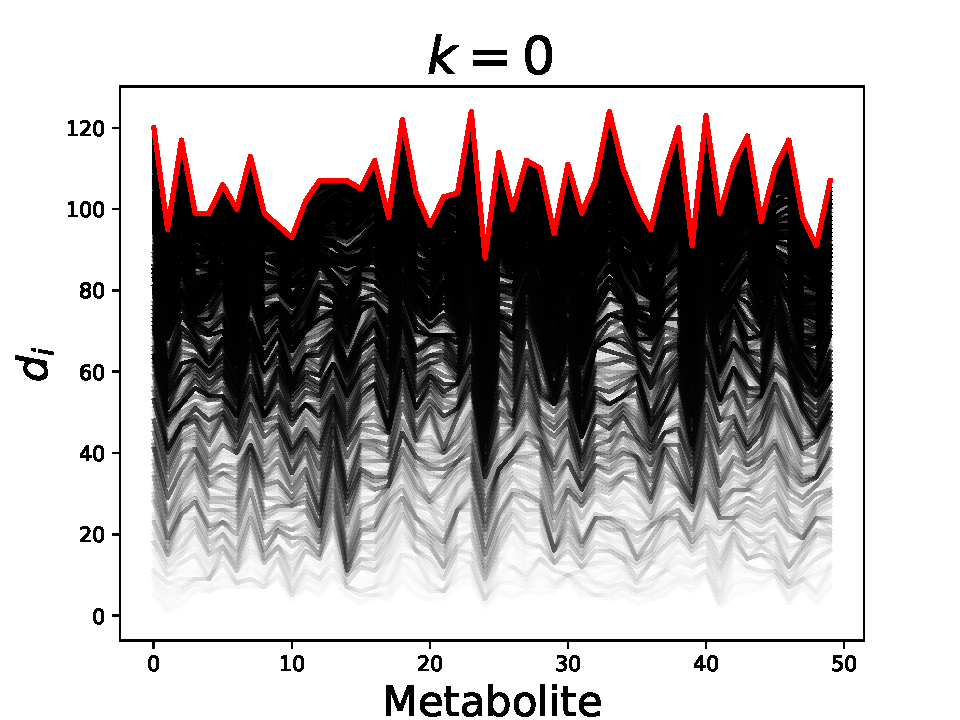
\includegraphics[width=.5\textwidth]{competition_k_0.pdf}\hfill
		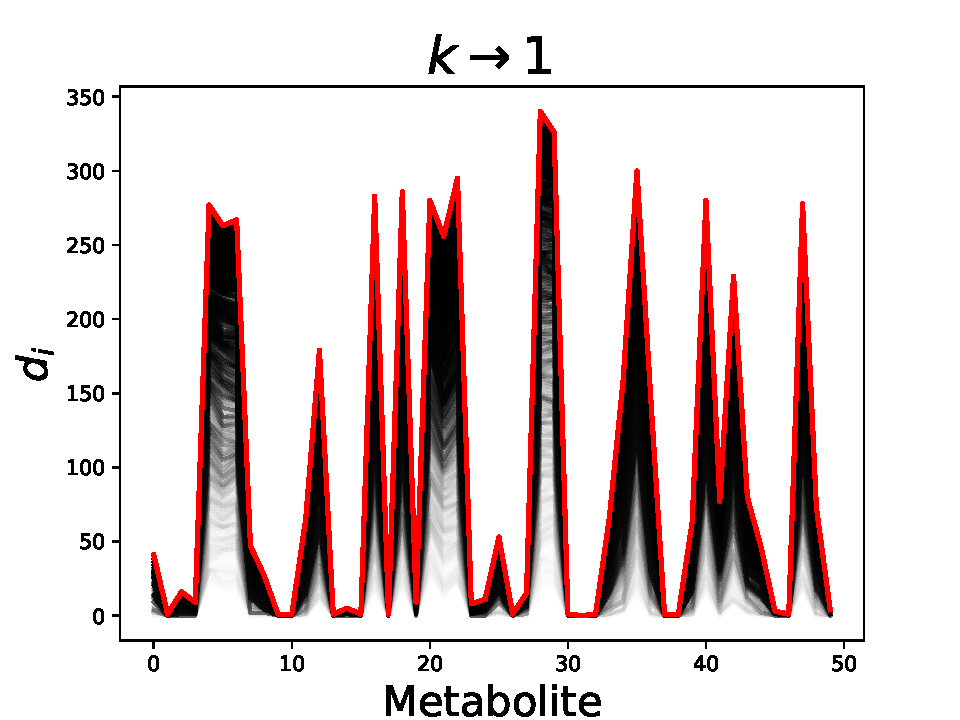
\includegraphics[width=.5\textwidth]{competition_k_1.pdf}
		\caption{Cumulative demand of each metabolite at each iteration for three characteristic values of $ k_c $. Visually inspecting the demand profile when the sampling is completed (red line), one verifies that competition is minimized for $ k_c \rightarrow -1 $ (left),  it is uniformly random for $ k_c = 0 $ (center), and is maximized when $  k_c \rightarrow 1$ (right).}
		\label{demand_profiles}
	\end{figure}

	Second, let me consider the problem of modulating the facilitation level of the community by sampling the metabolic cross-feeding topology, encoded in the community metabolic matrix $ D $. Each element of the metabolic matrix, $ D_{jk} $, specifies the fraction of leaked energy from resource $ j $ that is released in the form of resource $ k $. Note that by definition $ \sum_jD_{jk} = 1 $.\\ 
	I construct the matrix element $ D_{jk} $ is constructed by adding two terms. First, the $ k^{th} $ element of a random vector following a flat Dirichlet distribution, $ \vec{x_j} \sim Dir(\vec{\alpha})$ where all elements of the parameter vector $ \vec{\alpha} $ are equal to one, $ \alpha_k = 1 $. In this case, the Dirichlet distribution is equivalent to a uniform distribution over the standard ($ k  - 1 $)-simplex, where $ k \in \{1, \dots, m\} $. Second, a term that depends on the difference in demand between resources $ j $ and $ k $, that is, on $ d_{sj} - d_{sk}$, where $ s $ is the number of species (ommited from now on to avoid cluttering the notation). Let $ \Delta_{jk} $ denote the truncated difference between demands of resource $ j $ and $ k $ as
	\begin{equation}
		\Delta_{jk} = 
			\begin{cases}
				d_k - d_j & \text{ if } d_k > d_j\\
				1 & \text{ if } d_k = d_j\\
				0 & \text{ if } d_k < d_j\\
			\end{cases}
	\end{equation}
	Then, the fraction of the leaked resource $ j $ that is released in the form of resource $ k $ is given by
	\begin{equation}\label{sampling_metabolism}
		D_{jk} = (1-k_f)x_{jk} + k_f\frac{\Delta_{jk}}{\sum_j\Delta_{jk}}
	\end{equation}
	The weight of each term in equation \ref{sampling_metabolism} (the uniform random term, and the resource demand dependent term) is now modulated by $ k_f \in [0, 1]$, the facilitation factor. When $ k_f = 1 $, the first term  vanishes, and facilitation is maximized. Hence, more coveted metabolites are released at higher fractions. When $ k_f = 0 $, facilitiation is uniformly random, as all metabolites are released with equiprobable fractions.\par
	To illustrate the sampling of $ D $, figure \ref{sampling_D} is provided, where the total facilitation of each metabolite for two extreme values of $ k_f $ is overlayed with the demand profile of the community  in the case of maximum competition ($ k_c \rightarrow 1 $).\\
	
	\begin{figure}
		\centering
		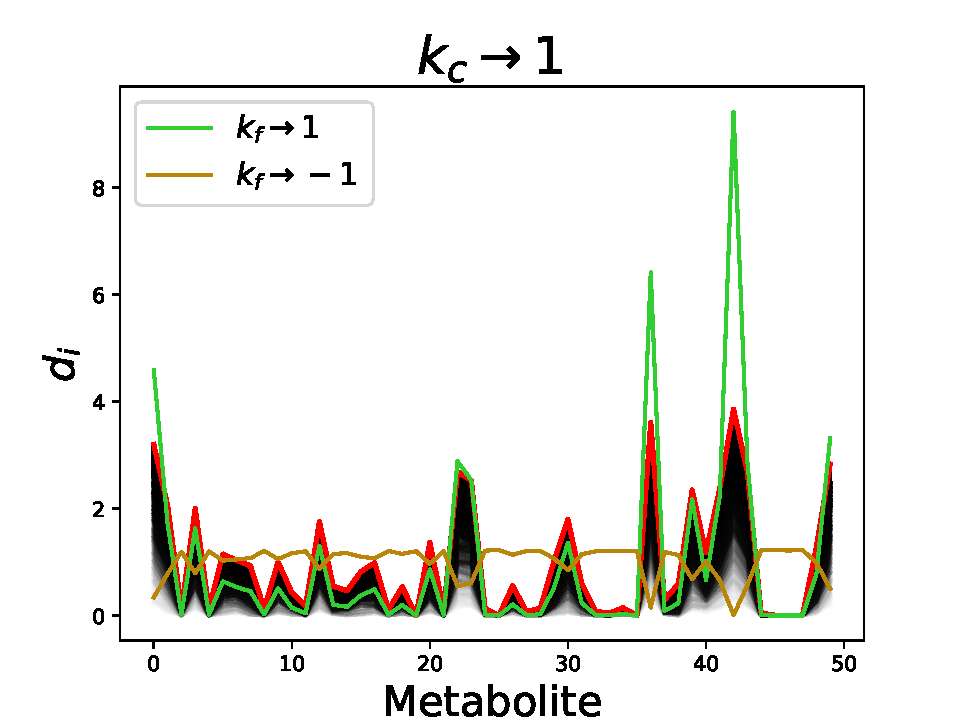
\includegraphics[width=\textwidth]{competition_facilitation_kf1_1_kc1.pdf}\hfill
		\caption{Rescaled demand profile for $ k_c \rightarrow 1 $and facilitation profile for the extreme values of $ k_f \rightarrow 1 $ and $ k_f \rightarrow -1 $}
		\label{sampling_D}
	\end{figure}
	Note that although the two methods for sampling $ c $ and $ D $ share similarities, they are conceptually different. First, the sampling of $ c $ is fully random, in the sense that a vector of probabilities is constructed first, and then preferences are randomly sampled from that distribution. On the other hand, the sampling of $ D $ has a random term, $ x_{jk} $, and a non-random term that depends only on the vector of demands of the community $ \vec{d_s} $. Another difference is that the competitiveness factor is imposed on the preference sampling probability vector, while the facilitation factor is imposed directly on the values of $ D $. Finally, the sampling of $ D $ depends on the sampling of $ c $, reflecting that high or low facilitation levels are achieved by tuning the secretion structure of the community to be symmetric to the profile of demands, or independent from it, respectively.
	
	\section{Community-level competition and facilitation metrics}
	
	The competition between species $ i $ and $ i' $ is quantified by the intake fraction of the resources consumed by both species. This can be expressed simply by taking the scalar product of the resource preference vectors of each species. 
	\begin{equation}
		C_{ii'} = (1- l)\sum_{j}c_{ij}c_{i'j} =  (1-l) \boldsymbol{c}_i\boldsymbol{c}^T_{i'}
	\end{equation}
	Note that, $ l_j $ was kept constant throughout simulations and equal for each resource, so that $ l_j = l $.\\
	On the other and, the facilitation of resource $ k $ that species $ i $ provides to $ i' $ from the consumption of metabolite $ j $, is quantified by 
	\begin{equation}
	    F_{ii'} = l\sum_{jk}c_{i'j}D_{jk}c_{ik} = l\boldsymbol{c}_iD\boldsymbol{c}_{i'}^T
	\end{equation}
	To calculate cohesion of the community, I substract the competition minus the facilitation levels of the whole community, which are obtained by averaging the values of competition and facilitation across all species pairs.
	\begin{equation}
	    \Theta = \langle C_{ii'} \rangle - \langle F_{ii'} \rangle
	\end{equation}
    \section{Coalescence event of two communities}
    Such event is simulated by mixing the species from each community after the assembly process in isolation has been completed. This can be mathematically expressed through a system of $ s_1 + s_2 + m $ differential equations, where $ s_1 $ and $ s_2 $ are the number of species that remain in the first and second communities after their assembly, respectively. 
    In matrix form, the system of two coalescing communities can be expressed as
    \begin{equation}\label{extended_system}
		\begin{aligned}
		\frac{d\boldsymbol{n}_e}{dt} &= \boldsymbol{g}\circ \boldsymbol{n}_{e}\left(D(\boldsymbol{R})C_{e}(\boldsymbol{1}-\boldsymbol{l}_e) - \boldsymbol{m}_e\right)\\
		\frac{d\boldsymbol{R}}{dt} &= \boldsymbol{\kappa} - D(\boldsymbol{R})\boldsymbol{\tau}^{\circ -1}- D(\boldsymbol{R})C_e^T\boldsymbol{n_e} + \left[\mathbb{1} \ \mathbb{1}\right] D_e^TD(\boldsymbol{l_e}\circ \boldsymbol{R_e})C_e^T\boldsymbol{n}_e
		\end{aligned}
	\end{equation}
	Where $ \left[\mathbb{1} \ \mathbb{1}\right] $ represents the horizontal concatenation of two $m \times m$ identity matrices. The sub-index $e$ stands for \textit{extended}. To form any of the extended vectors in equation \ref{extended_system}, one simply vertically concatenates the vectors from community 1 and community 2. Constructing an extended matrix in equation \ref{extended_system} is done by joining the two matrices alongside their diagonal. For example, constructing the vector of species abundances $\boldsymbol{n}_e$ and the metabolic matrix $D_e$ would be done as
	\begin{equation}
	    \boldsymbol{n}_e = \begin{bmatrix}
                                \boldsymbol{n}^{(1)} \\
                                \boldsymbol{n}^{(2)} \\
                            \end{bmatrix} 
        \qquad \qquad \qquad 
        D_e = \begin{bmatrix}
                    D^{(1)} & 0 \\
                    0 & D^{(2)} \\ 
              \end{bmatrix}
	\end{equation}
	where the superscripts indicate belonging to community 1 or 2
	\newpage
	\bibliographystyle{agsm}
	\bibliography{library}

\end{document}